\chapter{An evaluation of Wifi positioning accuracy} 

Up to this point in our paper we have discussed the steps that have been
taken in order to extract and analyze locations from Wifi data. The aim of the
current chapter is to present the steps we have taken in order to evaluate the
Wifi positioning in comparison to solutions that relay on GPS data.

The evolution of technology during the present days allows us to make use of
devices that register and process high amounts of contextual information about
their owners. Among these devices we can find our smartphones. Smartphones have
become a commodity without which we can hardly imagine our day to day life. We
use them for connecting and communicating with our friends, we use them for
recreational activities such as ``surfing'' the web, or in order to keep
ourselves up to date with the news in various domains that have captured our
interest. However, aside from allowing us to access all these types of
information while connecting us with the world around us, our smartphones have
another ability which not so many of us completely understand. They can collect
a large amount of contextual information about us. A strong example of how such
information can be used in the interest of the mobile phone's owner is provided
by the Google Now~\footnote{Further information at
http://www.google.com/landing/now/\#whatisit} service. This service uses various
contextual information that we make available through our Android phones in
order to provide us with important information like traffic statistics for when
we are expected to travel, weather information for the destination we should be
arriving at, or news about our favorite television show.

An example of contextual information that can be retrieved from our smartphones
is our locations, or our traveling patterns. This is possible due to the GPS
positioning that our smartphones allow. There are numerous studies which focus
on the possibility of extracting human mobility patterns from the GPS data
provided by mobile phones; among these studies we find
\cite{Montoliu:2010:DHP:1899475.1899487},
\cite{cuttone2014inferring},
\cite{Zhou:2007:DPM:1247715.1247718}, \cite{Ashbrook:2003:UGL:945305.945310}.

The database from SensibleDTU (Section~\ref{sensible_dtu}) contains, as it has
been mentioned previously, numerous types of information among which we can also
find GPS coordinates of the users that have accepted to be part of the
scientific project. For the present study, we had the opportunity to employ part
of this data in order to compare the results we obtain about the user locations
from their Wifi data with possible stop locations provided from their GPS data.

\section{Extracting stop locations from GPS data}

There are different algorithm that can be used for extracting stop locations
from GPS data. We present the three solutions that have been
explored in \cite{cuttone2014inferring} and which we have taken into
considerations as possibilities for extracting the stop locations.

\subsection{Speed thresholding}

This method relays on the calculation of speed in order to estimate if the data
represents a stop location or a movement. The approximation of the speed between
two given positions is calculated in this case as

\begin{equation}
Speed_{i} = \frac{Distance(pos_{i-1},pos_{i})}{timestamp_{pos_{i}}-timestamp_{pos_{i-1}}}
\end{equation}

Based on the given dataset and the frequency of sampling, the calculated speeds
can oscillate a lot. In \cite{cuttone2014inferring} the proposed solution for
this problem is to have the data grouped into time bins of a given size and to
consider that the position which corresponds to each time bin is given by the
median of the samples in the bin, thus allowing the calculation of the speed
between the bins instead of the samples. 

After the speeds are calculated, the samples for which a high speed~\footnote{A
speed is considered to be high if it is above a defined $Speed_{max}$ value} is
identified can be discarded as they can represent movement. The remaining
samples can be, therefor, associated to stop locations and can be grouped into
different stop locations. 

\subsection{Gaussian Mixtures Model}

A different approach presented in \cite{cuttone2014inferring} for grouping
samples into stop locations is to observe the overall distribution of the
existing samples without taking into consideration the timestamps. The idea is
to observe the clusters that form and to consider as stop locations the clusters
of samples which have a higher density.

The clusters are created by using a Gaussian Mixtures Model that attributes
samples to different clusters which are modeled as Gaussian distributions which
have unknown parameters. After a sample is allocated to a cluster, consecutive
samples that have been assigned to the same cluster can be grouped and consider
to form stop locations. The size of the clusters are determined by a given
parameter.
 
\subsection{Distance grouping}

The main idea behind the distance grouping algorithm, as it has been presented
in \cite{cuttone2014inferring}, is that a sequence of location samples which
seem to be geographically close to each other~\footnote{The location samples have
been identified within a given maximum distance $D_{max}$ of each other} can be
grouped into a stop location.

The stop locations are created as follows:
\begin{itemize}
  \item The samples are taken into consideration in the ascending order of their
  timestamps
  \item A stop location has initially only one location sample $L_{i}$
  attributed to it
  \item All the following $k$ samples as long as all samples $j \in \{i+1, k\}$
  respect the condition $Distance(L_{j}, L_{i}) < D_{max}$ are added to the
  location
  \item The process of constructing the next stop location is started again from
  location $L_{i+k+1}$
\end{itemize}

\section{Comparing results obtained with distance grouping algorithm}

For the purpose of analysing the locations we have obtained from the Wifi data
we have implemented the \textit{distance grouping algorithm}. Our implementation
considers that the maximum distance $D_{max}$ that determines the way in which
GPS samples are grouped is of $60$ m. The way in which this value is selected
affects the results as a very large large value for $D_{max}$ leads to the
merging of different stop locations while a very small value leads to stop
locations being unnecessarily divided into more smaller stop locations. The $60$
m value has proved to be a good approximation as it has been determined
empirically from the data that it provides acceptable results.

We also try to be consistent with the fact that for the Wifi data we consider
that a user needs to be close to a given geographical location for at least $5$
minutes in order for it to be considered a stop location and not a transition
location. In order to keep this assumption for the locations extracted from the
GPS data, we discard the stop locations for which the user does not seem to be
spending at least $5$ minutes within their limits. To calculate the time the
user spends in a GPS identified stop location we calculate the difference
between the timestamps of the first sample that is associated with the position
and the last sample that is still considered a part of the stop location. If the
difference is equal or above $5$ minutes, the stop location is kept.

Fig.~\ref{loc_wifi_data} represents a quantitative measurement for the number of
locations that a group of $65$ users change during a period of $30$ days
according to the Wifi data, while Fig.~\ref{loc_gps_data} represent a
quantitative measurement for the number of locations the same group of users
changes during the same period of time according to the GPS data. As we can see,
by using the GPS data we can identify a biger number of locations for a given
time frame than by using the Wifi data. The average number of locations changed
during a month per user according to the GPS data is approximately $153$, while
the average number identified for Wifi data is approximately $80$. Considering
these results we wanted to take a look at a time frame from the perspective of
the locations identified with both Wifi and GPS data in order to understand the
differences between the estimations.

\begin{figure}[!h]
\centering
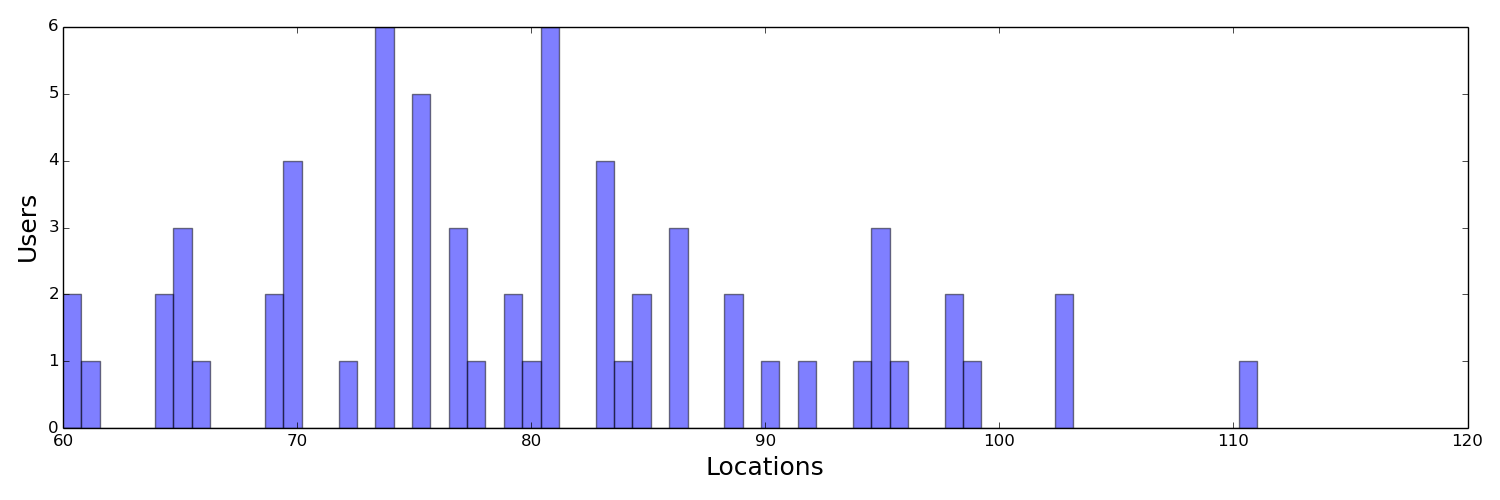
\includegraphics[width=\textwidth]{figures/gps/distribution_loc_wifi.png}
\caption{Count of location changes done during $30$ days by $65$ users
according to Wifi data}
\label{loc_wifi_data}
\end{figure}

\begin{figure}[!h]
\centering
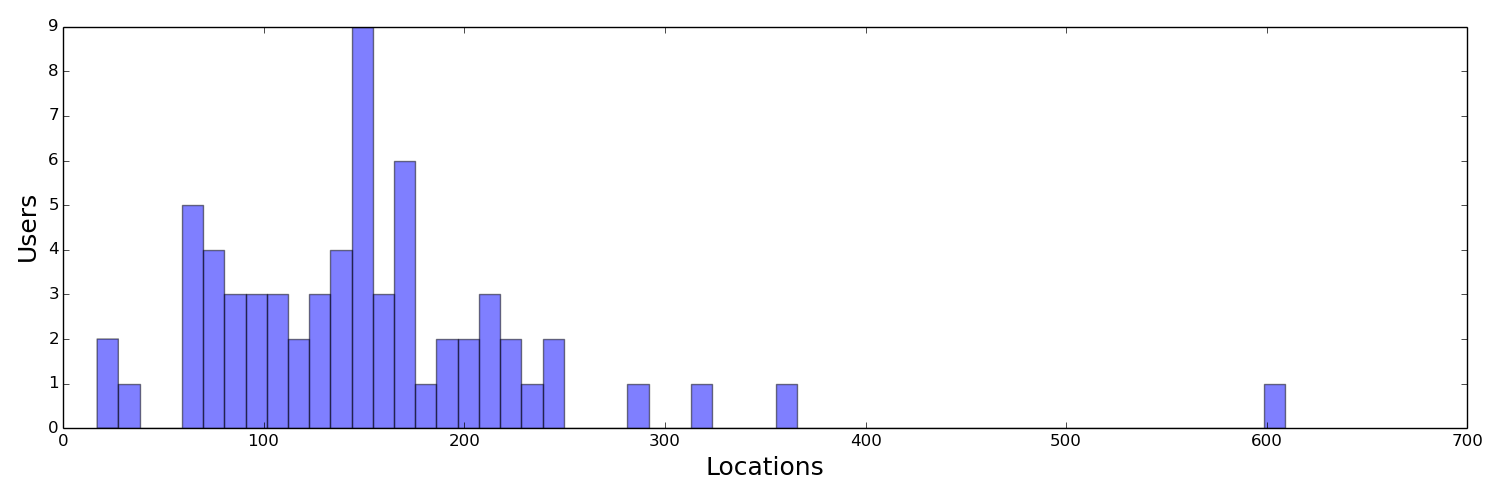
\includegraphics[width=\textwidth]{figures/gps/distribution_loc_gps.png}
\caption{Count of location changes done during $30$ days by $65$ users
according to GPS data}
\label{loc_gps_data}
\end{figure}

In Fig.~\ref{user6_aps_2days} we can see the predominant APs that have been
scanned during a $2$ days time frame for an user. Fig.~\ref{user6_hmm_2days}
displays the locations identified considering the Wifi data (first line of
colors) and the locations extracted from the GPS data (second line of colors).

\begin{figure}[!h]
\centering
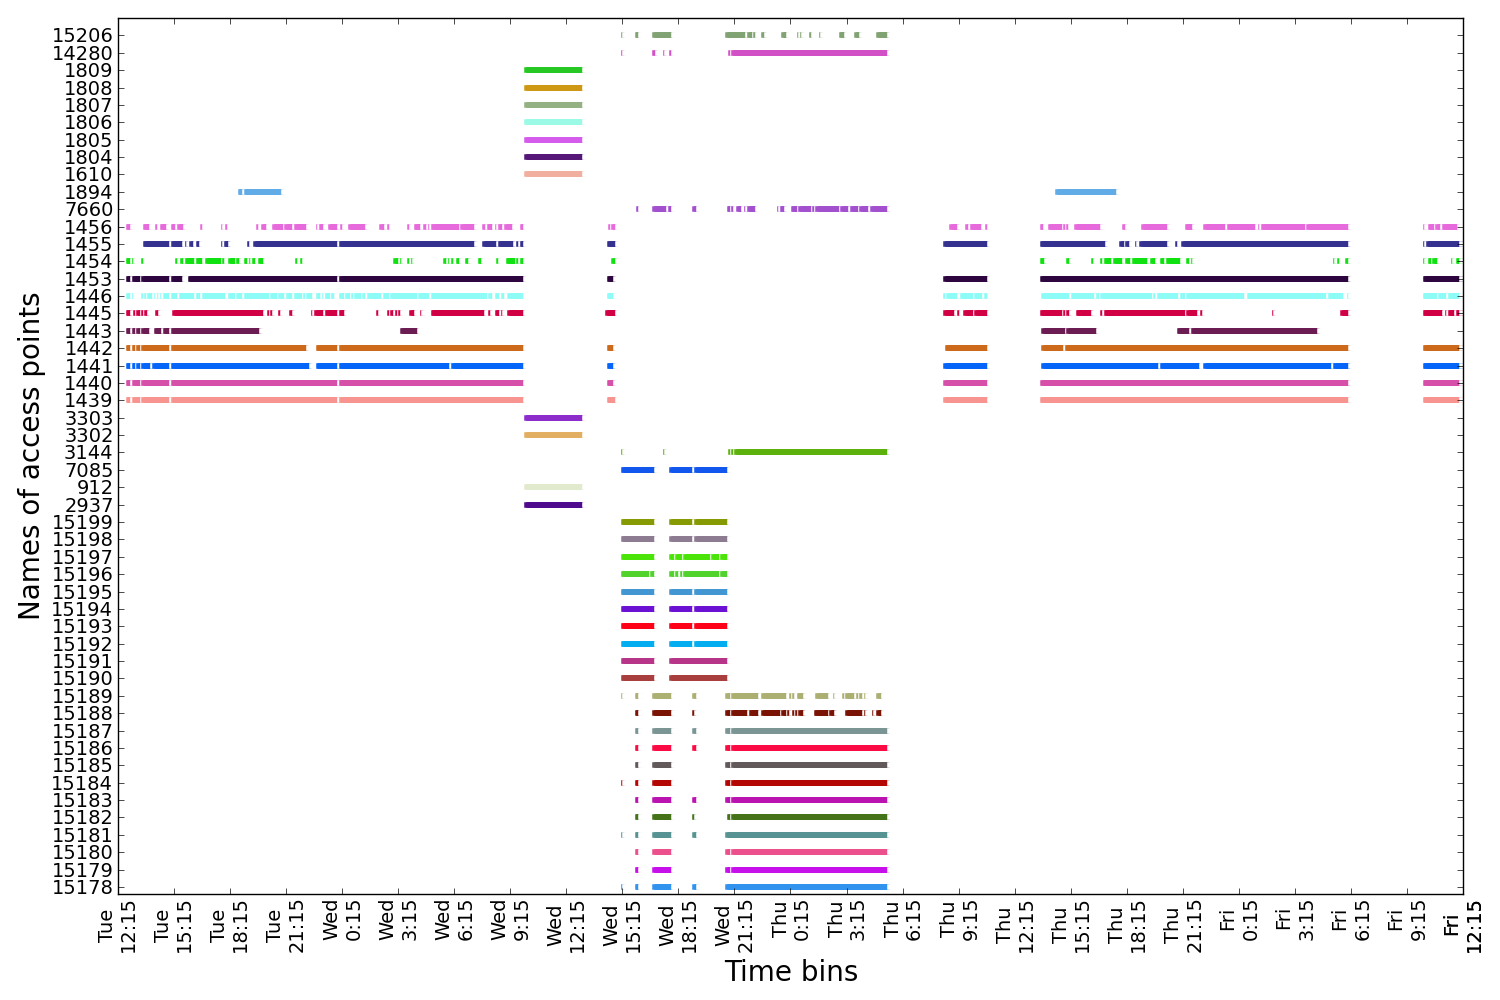
\includegraphics[width=\textwidth]{figures/gps/user_6_sorted_3days_no_rssi_plot.png}
\caption{The most common 50 APs for userX during 3 days scan records}
\label{user6_aps_2days}
\end{figure}

\begin{figure}[!h]
\centering
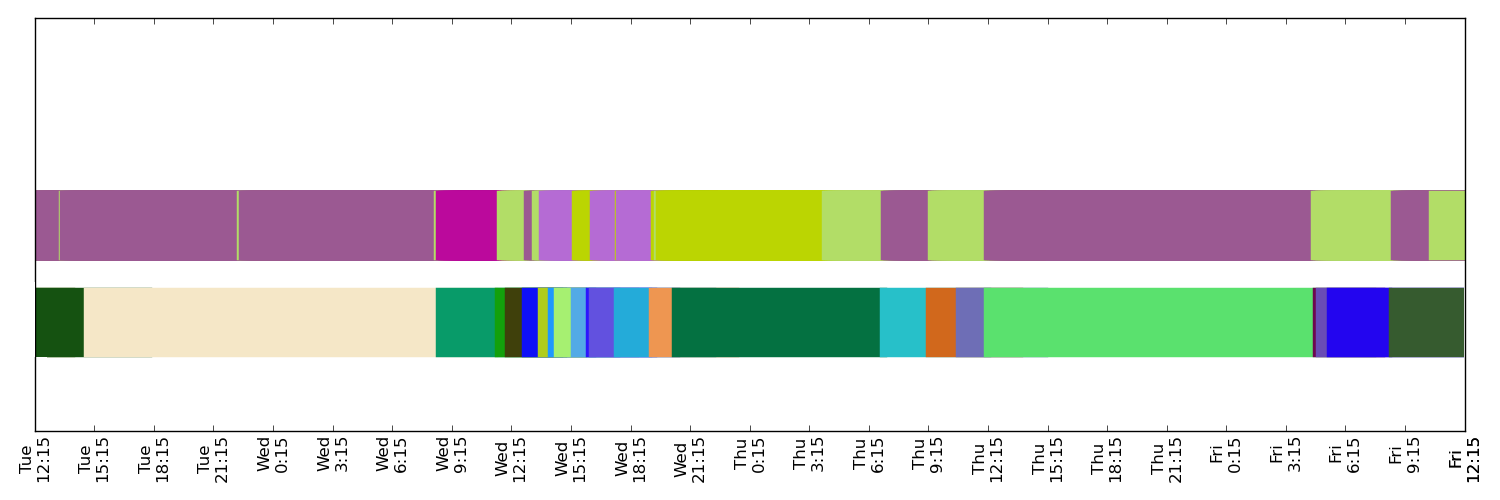
\includegraphics[width=\textwidth]{figures/gps/user_6_hmm_and_gps.png}
\caption{Wifi and GPS locations identified for userX throughout 3 days}
\label{user6_hmm_2days}
\end{figure}

From these images we can observe that the GPS data has, indeed, a better
accuracy when dealing with locations. For example, from the GPS data we can
identify that from Thursday morning and up to Thursday at noon, the user is
recorder to have changed location three times. In the Wifi data, only two
locations are identified withing the same time frame. A reason why this can be
possible is that the stop locations identified from GPS data are grouped
together if they are less than $60$ meters apart, while the Wifi stop locations
are calculated based on the visibility of the Wifi APs. In this case, if some
APs have a range of visibility which extends $60$ m, stop locations which can be
identified as being different based on GPS can be considered the same based on
Wifi data.

Despite some differences, the two figures do present similarities and are
clearly associated to the same time frame and the same user (for example, the
time between Thursday at around $12.15$ until Friday at around $4.00$ is
identified in both data as one stop location). However, the need for further
work in order to improve the way in which we estimate locations based on Wifi
data is needed. In this sense, an analysis of stop durations for both Wifi
and GPS data and an analysis of the fraction of stops that approximately overlap
can be a good starting point for further research.
